\documentclass[12pt]{article}

%\usepackage{graphics}
\usepackage{graphicx}
\usepackage{caption}
\usepackage{subcaption}
%\usepackage{epsfig}
%\usepackage{times}
%\usepackage{amsmath}
%\usepackage[spanish]{babel}
%\usepackage{lscape}
%\usepackage[nottoc,numbib]{tocbibind}
%\usepackage{pdfpages}

\title{Exercise 3}
\date{\today}
%\author{Mat\'{\i}as Rivero}

\begin{document}
\maketitle

\section{Assignment}
In engineering, the stresses are one of the prinicipal variables which helps to predict the failure of a mechanical component, defined by a specific shape and material, and subjected to specific boundary conditions. The yield stress of a given material is the stress at which that material begins to deform plastically. This material property determines the limit of performance for mechanical components. In structural engineering this is a soft failure mode which doesn't normally cause catastrophic failure, but it can be consider as a limit value for the designing of mechanical components.

Finite element analysis helps to predict the stress distribution of a mechanical piece under certain boundary conditions. This is of great help for the engineer during the design process. As the cost of performing a computer simulation of a given mechanical component is low compared with experiments, the engineer has the oportunity to redesign several times a specific component and evaluate its performance until all usage requeriments are fullfiled. 

\medskip

Let's consider a hook made of steel, subjected to Dirichlet (fixed end) and Neumann (load) boundary conditions. The geometry, material properties and boundary conditions are given by Fig.~\ref{fig:geometry}.
\begin{itemize}
\item Run this problem using Ostero and postprocess the results with ParaView.
\item Using ParaView, look for the point of maximum stress (to do this, split horizontally the Layout, create a SpreadSheet View and sort the SIGXX and SIGYY variable).
\item Regarding steel, its yield point is about 50 MPa. Considering the geometry and boundary conditions given, will this particular case behave under desired engineering limits?
\item If the answer is yes, explain why.
\item If the answer is no, as you are the mechanical designer, propose two solutions. Take into account that the boundary conditions can not be modified. Which solution is the cheapest? 
\end{itemize}

\vspace{2cm}

\begin{figure}[htp]
\begin{center}
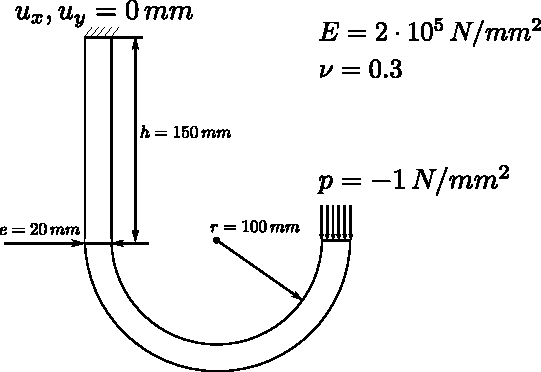
\includegraphics[width=0.8\linewidth]{hook.pdf}
\caption{Geometry, material properties and boundary conditions.}
\label{fig:geometry}
\end{center}
\end{figure}

\vspace{2cm}

\hrulefill


%~\cite{bib:belytschko}.
%\begin{thebibliography}{9}
%\bibitem{bib:belytschko} {\it Nonlinear Finite Elements for Continua and Structures}. Ted Belytschko, Wing Kam Liu, Brian Moran. Wiley, 2000. 
%\end{thebibliography}

\end{document}
